\setcounter{section}{0}
%\chapter[Động năng, thế năng]{Động năng, thế năng}
\section{Lý thuyết}
\subsection{Động năng}
\subsubsection{Khái niệm động năng}
Động năng của một vật là năng lượng mà vật có được do nó đang chuyển động. 

Nếu vật khối lượng $m$ đang chuyển động với vận tốc $v$ thì động năng của vật được xác định theo công thức:
\begin{equation*}
	W_{\text{đ}} =\dfrac{1}{2}mv^2.
\end{equation*}
\subsubsection{Đặc điểm của động năng}
\begin{itemize}
	\item Động năng là đại lượng vô hướng, không âm.
	\item Động năng có giá trị phụ thuộc vào hệ quy chiếu (do tính tương đối của vận tốc).
	\item Trong hệ SI, động năng có đơn vị là joule (J). 
\end{itemize}
\subsubsection{Định lý động năng}
Độ biến thiên động năng của một vật bằng công của ngoại lực tác dụng lên vật:
\begin{equation*}
	A_{12} = W_{\text{đ}_2}-W_{\text{đ}_1}= \dfrac{1}{2}mv^2_2-\dfrac{1}{2}mv^2_1,
\end{equation*}
trong đó:
\begin{itemize}
	\item $A_{12}$ là công của lực tác dụng,
	\item $W_{\text{đ}_2}$ là động năng lúc sau của vật,
	\item $W_{\text{đ}_1}$ là động năng lúc đầu của vật.
\end{itemize} 

\noindent Từ công thức của định lý động năng, ta rút ra nhận xét:
\begin{itemize}
	\item Công phát động $(A_{12}>0$) làm cho vận tốc của vật tăng nên $W_{\text{đ}_2} > W_{\text{đ}_1}$.
	\item Công cản $(A_{12}<0)$ làm cho vận tốc của vật giảm nên $W_{\text{đ}_2} < W_{\text{đ}_1}$.
\end{itemize}
\subsection{Thế năng trọng trường}
\subsubsection{Khái niệm thế năng trọng trường}

Thế năng trọng trường của một vật là dạng năng lượng tương tác giữa Trái Đất và vật, phụ thuộc vào vị trí của vật trong trọng trường.	
\begin{center}
	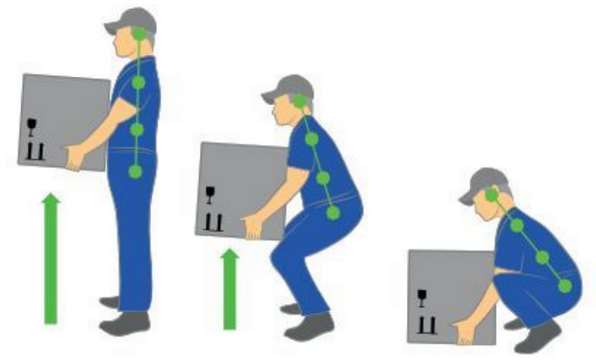
\includegraphics[scale=0.4]{../figs/G10-020-1}
\end{center}
\subsubsection{Biểu thức thế năng trọng trường}

Thế năng phụ thuộc vào vị trí của vật đối với vị trí được chọn làm mốc thế năng. 

Nếu chọn mốc thế năng trên mặt đất, khi một vật có khối lượng $m$ đặt ở độ cao $z$ so với mặt đất (trong trọng trường của Trái Đất) thì thế năng trọng trường của vật được xác định bằng công thức
\begin{equation*}
	W_\text{t}=mgz;
\end{equation*}
trong đó:
\begin{itemize}
	\item $W_\text{t}$ là thế năng trọng trường (có đơn vị là J);
	\item $m$ là khối lượng (có đơn vị là kg);
	\item $z$ là độ cao của vật so với mặt đất (có đơn vị là m).
\end{itemize}
Thế năng của vật trên mặt đất (vị trí mốc thế năng) bằng 0 ($z=0$). 

\subsubsection{Đặc điểm của thế năng trọng trường}

\begin{itemize}
	\item Thế năng là một đại lượng vô hướng có giá trị dương hoặc âm hoặc bằng không;
	\item Thế năng có tính tương đối, nghĩa là thế năng phụ thuộc vào vị trí ta chọn làm gốc thế năng;
	\item Trong bài toán chuyển động của vật, ta thường chọn gốc thế năng là tại mặt đất hoặc vị trí thấp nhất trên quỹ đạo của vật.
\end{itemize}

\ppgiai{
	\begin{description}
		\item[Bước 1:] Chọn gốc thế năng;
		\item [Bước 2:] Xác định giá trị đại số độ cao $z$ của vật so với mốc thế năng;
		\item [Bước 3:] Xác định thế năng của vật theo biểu thức
		\begin{equation*}
			W_\text{t}=mgz.
		\end{equation*}
	\end{description}
}
\subsubsection{Liên hệ giữa biến thiên thế năng và công của trọng lực}

Khi một vật chuyển động trong trọng trường từ vị trí M đến vị trí N thì công của trọng lực của vật có giá trị bằng hiệu thế năng trọng trường tại M và N
\begin{equation*}
	A_\text{MN}=W_{\text{tM}}-W_{\text{tN}};
\end{equation*}
trong đó:
\begin{itemize}
	\item $A_\text{MN}$ là công của trọng lực;
	\item $W_{\text{tM}}$ và $W_{\text{tN}}$ lần lượt là thế năng tại M và thế năng tại N.
\end{itemize}

\textit{Hệ quả:} Trong quá trình chuyển động của một vật trong trọng trường:

\begin{itemize}
	\item Khi vật giảm độ cao, thế năng của vật giảm thì trọng lực sinh công dương.
	\item Khi vật tăng độ cao, thế năng của vật tăng thì trọng lực sinh công âm.
\end{itemize}

\ppgiai{
	\begin{description}
		\item [Bước 1:] Xác định lực (hợp lực) tác dụng vào vật;
		\item [Bước 2:] Xác định công của lực (hợp lực) tác dụng vào vật;
		\item [Bước 3:] Viết biểu thức biến thiên cơ năng
		\begin{equation*}
			A=W_{\text{t}1}-W_{\text{t}2};
		\end{equation*}
		\item [Bước 4:] Xác định các đại lượng theo yêu cầu của đề bài.
	\end{description}
}

\section{Mục tiêu bài học - Ví dụ minh họa}
\begin{dang}{Tính động năng của một vật}
	\viduii{2}{Một vật có khối lượng $\SI{0.5}{kg}$ chuyển động với vận tốc $\SI{10}{m/s}$. Động năng của vật bằng
		\begin{mcq}(4)
			\item $\SI{250}{J}$.
			\item $\SI{50}{J}$.
			\item $\SI{5}{J}$.
			\item $\SI{25}{J}$.
		\end{mcq}
	}
	{	\begin{center}
			\textbf{Hướng dẫn giải}
		\end{center}
		Động năng của vật: $W_\text{đ} = \dfrac{1}{2}mv^2 =\dfrac{1}{2}\cdot\SI{0.5}{\kilogram}\cdot(\SI{10}{\meter/\second})^2= \SI{25}{J}$.
		
		\textbf{Đáp án: D.}
		
		\begin{center}
			\textbf{Câu hỏi tương tự}
		\end{center}
		
		Một vật có khối lượng $\SI{250}{g}$ đang di chuyển với tốc độ $\SI{10}{m/s}$. Động năng của vật này là
		\begin{mcq}(4)
			\item $\SI{12.5}{J}$.
			\item $\SI{25}{J}$.
			\item $\SI{12500}{J}$.
			\item $\SI{25000}{J}$.
		\end{mcq}
		
		\textbf{Đáp án:} A.
	}
	\viduii{2}{Một vận động viên có khối lượng $\SI{80}{kg}$ chạy đều hết quãng đường $\SI{180}{m}$ trong thời gian 40 giây. Động năng của vận động viên đó là
		\begin{mcq}(4)
			\item $\SI{810}{J}$. 
			\item $\SI{360}{J}$.
			\item $\SI{875}{J}$.
			\item $\SI{180}{J}$.
		\end{mcq}
	}
	{	\begin{center}
			\textbf{Hướng dẫn giải}
		\end{center}
		
		Vận tốc của vận động viên:
		$$v=\dfrac{s}{t} =\dfrac{\SI{180}{\meter}}{\SI{40}{\second}}= \SI{4.5}{\meter/\second}.$$
		
		Động năng của vận động viên:
		$$W_\text{đ} = \dfrac{1}{2} mv^2 =\dfrac{1}{2}\cdot\SI{80}{\kilogram}\cdot(\SI{4.5}{\meter/\second})^2= \SI{810}{J}.$$
		
		\textbf{Đáp án: A.}
		
		
		\begin{center}
			\textbf{Câu hỏi tương tự}
		\end{center}
		
		Một vật có khối lượng 500 g rơi tự do từ độ cao $z$ = 100 m xuống đất, lấy $g = 10\ \text{m/s}^2$. Động năng của vật tại độ cao 50 m so với mặt đất bằng bao nhiêu?
		
		\textbf{Đáp án:} $250\ \text{J}$.
		
		
	}
\end{dang}

\begin{dang}{Biện luận giá trị động năng khi thay đổi các đại lượng}
	\viduii{2}{Một viên đạn khối lượng 10 g bay ra từ nòng súng với vận tốc 600 m/s và một vận động viên khối lượng 58 kg chạy với vận tốc 8 m/s. Hãy so sánh động năng của người và đạn.
	}
	{	\begin{center}
			\textbf{Hướng dẫn giải}
		\end{center}
		
		Động năng của đạn
		\begin{equation*}
			\dfrac{1}{2}mv^2=\dfrac{1}{2}\cdot\SI{0.01}{\kilogram}\cdot(\SI{600}{\meter/\second})^2 =1800\ \text{J}.
		\end{equation*}	
		
		Động năng của người 
		\begin{equation*}
			\dfrac{1}{2}MV^2 =\dfrac{1}{2}\cdot\SI{58}{\kilogram}\cdot(\SI{8}{\meter/\second})^2=1856\ \text{J}.
		\end{equation*}
		
		Mặc dù khối lượng của đạn rất nhỏ so với khối lượng người, nhưng động năng của đạn và người xấp xỉ bằng nhau. Điều đó chứng tỏ yếu tố vận tốc có ảnh hưởng mạnh đối với giá trị động năng.
		
		\begin{center}
			\textbf{Câu hỏi tương tự}
		\end{center}
		
		Hãy so sánh động năng của một chiếc mô tô chạy quá tốc độ ở $\SI{120}{km/h}$ với động năng của chính nó ở tốc độ thông thường là $\SI{40}{km/h}$. Từ đó cho nhận xét về mức độ nguy hiểm của việc chạy quá tốc độ.
		
		\textbf{Đáp án:} $W_\text{đ2} = 9W_\text{đ1}$.
	}
	%	\viduii{2}{
		%		Khi vận tốc của vật tăng gấp đôi thì
		%		\begin{mcq}(2)
			%			\item động lượng của vật tăng gấp đôi.
			%			\item gia tốc của vật tăng gấp đôi.
			%			\item động năng của vật tăng gấp đôi.
			%			\item thế năng của vật tăng gấp đôi.
			%		\end{mcq}
		%	}
	%	{\begin{center}
			%			\textbf{Hướng dẫn giải}
			%		\end{center}
		
		%		Khi vận tốc của vật tăng gấp đôi thì động lượng của vật tăng gấp đôi, động năng của vật tăng gấp 4.
		
		%		\textbf{Đáp án: A}.
		
		%		\begin{center}
			%			\textbf{Câu hỏi tương tự}
			%		\end{center}
		
		%		Khi vận tốc của vật tăng gấp đôi, đồng thời khối lượng giảm đi một nửa thì
		%		\begin{mcq}(2)
			%			\item động lượng của vật tăng gấp đôi.
			%			\item gia tốc của vật tăng gấp đôi.
			%			\item động năng của vật tăng gấp đôi.
			%			\item thế năng của vật tăng gấp đôi.
			%		\end{mcq}
		
		%		\textbf{Đáp án: C}.
		%	}
\end{dang}
\begin{dang}{Tính độ biến thiên động năng}
	\viduii{2}{Một ô tô khối lượng $m$ bằng 1 tấn đang chuyển động với vận tốc $v=\SI{20}{m/s}$. Tính độ biến thiên động năng của ô tô khi nó bị hãm tới khi vận tốc còn $\SI{10}{m/s}$.
	}
	{	\begin{center}
			\textbf{Hướng dẫn giải}
		\end{center}
		Độ biến thiên động năng:
		\begin{align*}
			\Delta W_\text{đ} &= \dfrac{1}{2}mv^2-\dfrac{1}{2}mv_0^2\\
			&=\dfrac{1}{2}\cdot\SI{1000}{\kilogram}\cdot(\SI{10}{\meter/\second})^2-\dfrac{1}{2}\cdot\SI{1000}{\kilogram}\cdot(\SI{20}{\meter/\second})^2\\
			&= \SI{-150000}{J}=\SI{-150}{\kilo\joule}.
		\end{align*}
		
		
		\begin{center}
			\textbf{Câu hỏi tương tự}
		\end{center}
		
		Một ô tô có khối lượng 4 tấn đang chuyển động với vận tốc $\SI{36}{\kilo\meter/\hour}$ thì hãm phanh, sau một thời gian vận tốc giảm còn $\SI{18}{\kilo\meter/\hour}$. Độ biến thiên của động năng của ô tô là
		\begin{mcq}(4)
			\item $\SI{150}{\kilo\joule}$.
			\item $\SI{-150}{\kilo\joule}$.
			\item $\SI{-75}{\kilo\joule}$.
			\item $\SI{75}{\kilo\joule}$.
		\end{mcq}
		
		\textbf{Đáp án:} B.
	}
	\viduii{2}{Một lực $F$ không đổi làm một vật bắt đầu chuyển động và đạt được vận tốc $v$ sau khi đi được quãng đường $s$. Nếu tăng lực tác dụng lên 3 lần thì vận tốc của nó sẽ gấp bao nhiêu lần so với $v$? Cho biết quãng đường trong hai trường hợp đều là $s$.
	}
	{	\begin{center}
			\textbf{Hướng dẫn giải}
		\end{center}
		
		Áp dụng định lý động năng
		\begin{equation*}
			A=Fs= \dfrac{1}{2}mv^2-\dfrac{1}{2}mv_0^2 = \dfrac{1}{2}mv^2 \Rightarrow v =\sqrt{\dfrac{2  F  s}{m}}.
		\end{equation*}
		Biểu thức trên cho thấy vận tốc tỉ lệ với căn bậc hai của lực, do đó khi lực tăng lên 3 lần thì vận tốc tăng $\sqrt{3}$ lần.
		
		
		\begin{center}
			\textbf{Câu hỏi tương tự}
		\end{center}
		
		Một lực $F$ không đổi làm một vật bắt đầu chuyển động và đạt được vận tốc $v$ sau khi đi được quãng đường $S$. Nếu tăng lực tác dụng lên 3 lần đồng thời quãng đường cũng tăng lên 3 lần thì vận tốc của nó sẽ gấp bao nhiêu lần so với $v$ ở cuối quãng đường ấy?
		
		\textbf{Đáp án:} $v'=3v$.
	}
\end{dang}

\begin{dang}{Áp dụng định lí động năng}
	\viduii{3}{Một xe khối lượng 1 tấn khởi hành không vận tốc đầu, chuyển động nhanh dần đều trên đường nằm ngang. Sau khi đi được quãng đường $\SI{100}{m}$ thì đạt vận tốc $\SI{72}{km/h}$. Biết lực ma sát bằng $5\%$ trọng lượng của xe. Dùng định lý động năng, tính công của lực kéo của động cơ xe.
	}
	{	\begin{center}
			\textbf{Hướng dẫn giải}
		\end{center}
		
		Lực ma sát có độ lớn 
		$$F_\text{ms} = 5\%\cdot mg = 5\%\cdot\SI{1000}{\kilogram}\cdot\SI{10}{\meter/\second^2}=\SI{500}{N}.$$
		
		Áp dụng định lý động năng, độ biến thiên động năng bằng tổng công của các lực 
		\begin{align*}
			A_F + A_\text{ms} &= \dfrac{1}{2}mv^2 - 0\\ \Rightarrow\quad A_F &= \dfrac{1}{2} mv^2 - (-F_\text{ms}s) \\
			&=\dfrac{1}{2}\cdot\SI{1000}{\kilogram}\cdot(\SI{20}{\meter/\second})^2-(-\SI{500}{\newton}\cdot\SI{100}{\meter})\\
			&= \SI{250000}{J}\\
			&=\SI{250}{\kilo\joule}.		
		\end{align*}
		
		
		\begin{center}
			\textbf{Câu hỏi tương tự}
		\end{center}
		
		Một máy bay khối lượng $m = 5 \cdot 10^3\ \text{kg}$ bắt đầu chạy trên đường băng hết quãng đường dài 530 m thì đạt đến vận tốc cất cánh $v=60\ \text{m/s}$. Trong khi lăn bánh, lực cản trung bình bằng 0,02 trọng lượng của máy bay. Hãy xác định lực kéo của động cơ máy bay. Cho $g=10\ \text{m/s}^2$.
		
		\textbf{Đáp án:} $F = \text{1,8}\cdot 10^4\ \text{N}$.
	}
	\viduii{3}{
		Một ô tô có khối lượng 2 tấn đang chạy với vận tốc $\SI{54}{km/h}$ trên đường nằm ngang thì lái xe thấy có chướng ngại vật cách ô tô $\SI{100}{m}$ thì tắt máy, đạp thắng. Biết hệ số ma sát giữa bánh xe và mặt đường là $\mu = 0,1$. Xe ô tô có đâm vào chướng ngại vật không? Cho $g=\SI{10}{m/s^2}$.
	}
	{\begin{center}
			\textbf{Hướng dẫn giải}
		\end{center}
		Đơn vị vận tốc được đổi sang hệ SI $$\SI{54}{\kilo\meter/\hour}=\dfrac{\SI{54e3}{\meter}}{\SI{3600}{\second}}=\SI{15}{\meter/\second}.$$
		
		Lực ma sát có độ lớn 
		\begin{align*}
			F_\text{ms}=\mu mg=\SI{0.1}{}\cdot\SI{2000}{\kilogram}\cdot\SI{10}{\meter/\second^2}=\SI{2000}{\newton}.
		\end{align*}
		Quãng đường xe chạy được cho đến khi dừng hẳn theo lý thuyết định lý động năng là
		$$-F_\text{ms}s = 0 - \dfrac{1}{2}mv^2 \quad\Rightarrow\quad s = \dfrac{mv^2}{2F_\text{ms}}=\dfrac{\SI{2000}{\kilogram}\cdot(\SI{15}{\meter/\second})^2}{2\cdot\SI{2000}{\newton}}=\SI{112.5}{m}.$$
		
		Thực tế ô tô chỉ cách chướng ngại vật $\SI{100}{m}$ nên ô tô sẽ đâm vào chướng ngại vật trước khi kịp dừng lại.
		
		\begin{center}
			\textbf{Câu hỏi tương tự}
		\end{center}
		
		Một ô tô có khối lượng $\SI{1600}{\kilogram}$ đang chạy với tốc độ $\SI{54}{\kilo\meter/\hour}$ thì người lái xe nhìn thấy một vật cản trước mặt cách khoảng $\SI{10}{\meter}$. Người đó tắt máy và hãm phanh khẩn cấp với lực hãm không đổi là $\SI{2e4}{\newton}$. Xe dừng lại cách vật cản một khoảng bằng
		\begin{mcq}(4)
			\item $\SI{1,2}{\meter}$.
			\item $\SI{1,0}{\meter}$.
			\item $\SI{1,4}{\meter}$.
			\item $\SI{1,5}{\meter}$.
		\end{mcq}
		
		\textbf{Đáp án: B}.
	}
	\viduii{4}{
		Một ô tô có khối lượng 2 tấn đang chuyển động trên đường thẳng nằm ngang AB dài $\SI{100}{\meter}$, khi qua A vận tốc ô tô là $\SI{10}{\meter/\second}$ và đến B vận tốc của ô tô là $\SI{20}{\meter/\second}$. Biết độ lớn của lực kéo là $\SI{4000}{\newton}$.
		\begin{enumerate}[label=\alph*)]
			\item Tìm hệ số ma sát $\mu_1$ trên đoạn đường AB.
			\item Đến B thì động cơ tắt máy và lên dốc BC dài $\SI{40}{\meter}$ nghiêng $30^\circ$ so với mặt phẳng ngang. Hệ số ma sát trên mặt dốc là $\mu_2=\dfrac{1}{5\sqrt{3}}$. Hỏi xe có lên đến đỉnh dốc C không?
			\item Nếu đến B với vận tốc trên, muốn xe lên dốc và dừng lại tại C thì phải tác dụng liên tục lên xe một lực có độ lớn bao nhiêu?
		\end{enumerate}
	}
	{\begin{center}
			\textbf{Hướng dẫn giải}
		\end{center}
		
		\begin{enumerate}[label=\alph*)]
			\item 
			
			Áp dụng định lý động năng:
			$$-\mu_1 mg s_1 + Fs_1 = \dfrac{1}{2}mv_\text{B}^2 - \dfrac{1}{2}mv_\text{A}^2 \Rightarrow \mu_1 = \SI{0.05}{}.$$
			\item 			
			Áp dụng định lý động năng từ B đến khi xe dừng lại:
			$$A_\text{ms2}+A_{P2} = 0 - \dfrac{1}{2}mv_\text{B}^2 \Rightarrow -\mu_2 mg \cos \alpha s_2 - mgs_2 \sin \alpha = 0 - \dfrac{1}{2}mv_\text{B}^2 \Rightarrow s_2 = \SI{33.33}{m}.$$
			
			Vậy quãng đường tối đa xe lên được là $\SI{33.33}{m}$, mà dốc dài $\SI{40}{m}$ nên xe không lên được đến đỉnh dốc.
			\item 			
			Để xe lên được đến C thì $s_3=\SI{40}{m}$, khi đó:
			$$A_\text{ms3}+A_{P3}+A_F = 0 - \dfrac{1}{2}mv_\text{B}^2$$ $$\Rightarrow -\mu_2 mg \cos \alpha s_3 - mgs_3 \sin \alpha +Fs_3= 0 - \dfrac{1}{2}mv_\text{B}^2 \Rightarrow F = \SI{1}{N}.$$
		\end{enumerate}
	}
\end{dang}
\begin{dang}{Xác định thế năng của vật trong trọng trường}
	\viduii{2}{Một vật có khối lượng $\SI{2}{kg}$ được thả rơi từ độ cao $\SI{4.5}{m}$ xuống mặt đất, tại nơi có gia tốc trọng trường là $\SI{10}{m/s^2}$. Xác định thế năng của vật.
	}
	{	\begin{center}
			\textbf{Hướng dẫn giải}
		\end{center}
		Chọn gốc thế năng tại mặt đất. Thế năng của vật:
		$$W_\text t = mgz = \SI{2}{\kilogram}\cdot\SI{10}{\meter/\second^2}\cdot\SI{4.5}{\meter}=\SI{90}{J}.$$
		
		\begin{center}
			\textbf{Câu hỏi tương tự}
		\end{center}
		
		Thế năng của vật nặng $\SI{2}{\kilogram}$ ở đáy một giếng sâu $\SI{10}{\meter}$ so với mặt đất tại nơi có gia tốc $g= \SI{10}{\meter/\second^2}$ là bao nhiêu?
		\begin{mcq}(4)
			\item $\SI{-100}{\joule}$.
			\item $\SI{100}{\joule}$.
			\item $\SI{200}{\joule}$.
			\item $\SI{-200}{\joule}$. 
		\end{mcq}
		
		\textbf{Đáp án: D}.
	}
	\viduii{2}{Một vật có khối lượng $\SI{10}{\kilogram}$, lấy $\SI{10}{\meter/\second^2}$. Tính thế năng của vật tại A cách mặt đất $\SI{3}{m}$ về phía trên và tại đáy giếng B cách mặt đất $\SI{5}{m}$ với gốc thế năng tại mặt đất.
	}
	{	\begin{center}
			\textbf{Hướng dẫn giải}
		\end{center}
		
		Thế năng của vật tại A cách mặt đất $\SI{3}{m}$ ($z_\text{A}=\SI{3}{m}$) là
		\begin{equation*}
			W_{\text{tA}}=mgz_\text{A}=\SI{10}{\kilogram}\cdot\SI{10}{\meter/\second^2}\cdot\SI{3}{m}=\SI{300}{\joule}.
		\end{equation*}
		
		Thế năng của vật tại đáy giếng B cách mặt đất $\SI{5}{m}$ ($z_\text{B}=-\SI{5}{m}$) là
		\begin{equation*}
			W_{\text{tB}}=mgz_\text{B}=\SI{10}{\kilogram}\cdot\SI{10}{\meter/\second^2}\cdot(-\SI{5}{m})=\SI{-500}{\joule}.
		\end{equation*}
		
		
		\begin{center}
			\textbf{Câu hỏi tương tự}
		\end{center}
		
		Nếu lấy mốc thế năng tại đáy giếng, hãy tính lại kết quả câu trên.
		
		\textbf{Đáp án:} $\SI{800}{\joule}$; $0$.
	}
	\viduii{3}{Một học sinh thả một vật rơi tự do có khối lượng $\SI{500}{\gram}$ từ độ cao $\SI{45}{\meter}$ so với mặt đất, bỏ qua ma sát với không khí. Tính thế năng của vật tại giây thứ hai so với mặt đất. Cho $g= \SI{10}{\meter/\second^2}$.
	}
	{	\begin{center}
			\textbf{Hướng dẫn giải}
		\end{center}
		
		Độ cao của vật tại giây thứ hai so với mặt đất:
		$$h_2 = h - \dfrac{1}{2}gt^2 = \SI{25}{m}.$$
		
		Chọn gốc thế năng tại mặt đất. Thế năng của vật tại thời điểm đó:
		$$W_\text t = mgh_2 = \SI{0.5}{\kilogram}\cdot\SI{10}{\meter/\second^2}\cdot\SI{25}{\meter}=\SI{125}{J}.$$
		
		\begin{center}
			\textbf{Câu hỏi tương tự}
		\end{center}
		
		Với đề bài tương tự như trên, tính độ giảm thế năng của vật từ đầu giây thứ hai đến cuối giây thứ hai kể từ lúc thả.
		
		\textbf{Đáp án:} $\Delta W_\text{t} = \SI{75}{J}$.
	}
\end{dang}

\begin{dang}{Vận dụng liên hệ giữa công của trọng lực  và độ biến thiên thế năng }
	
	\viduii{2}{
		Một vật có khối lượng $\SI{100}{\gram}$ đang ở độ cao $\SI{6}{\meter}$ so với mặt đất. Tìm công của trọng lực tác dụng lên vật khi vật rơi đến độ cao $\SI{2}{\meter}$.
	}
	{\begin{center}
			\textbf{Hướng dẫn giải}
		\end{center}
		
		Chọn gốc thế năng tại mặt đất.
		
		Công của trọng lực tác dụng lên vật khi vật rơi từ độ cao $\SI{6}{\meter}$ đến độ cao $\SI{2}{\meter}$ là
		\begin{equation*}
			A=W_{\text{t}1}-W_{\text{t}2}=mgz_1-mgz_2=mg(z_1-z_2)=\SI{0,1}{\kilogram}\cdot\SI{10}{\meter/\second^2}\cdot(\SI{6}{\meter}-\SI{2}{\meter})=\SI{4}{\joule}.
		\end{equation*}
		
		\begin{center}
			\textbf{Câu hỏi tương tự}
		\end{center}
		
		Dùng lực để nâng vật có khối lượng $\SI{180}{g}$ thẳng đứng lên cao một đoạn $\SI{50}{cm}$. Tìm công của trọng lực trong quá trình trên. Lấy $g=\SI{10}{m/s^2}$.
		
		\textbf{Đáp án:} $\SI{-0.9}{J}$.
	}
	\viduii{3}{
		Một người thực hiện một công đạp xe đạp lên đoạn đường dài $\SI{40}{\meter}$ trên một dốc nghiêng $20^\circ$ so với phương ngang. Bỏ qua mọi ma sát. Nếu thực hiện một công cũng như vậy mà lên dốc nghiêng $30^\circ$ so với phương ngang thì người đó sẽ đi được đoạn đường bao nhiêu?
	}
	{\begin{center}
			\textbf{Hướng dẫn giải}
		\end{center}
		
		Chọn gốc thế năng tại mặt đất.
		
		Nếu bỏ qua mọi ma sát, thì công tối thiểu người này cần thực hiện lên dốc bằng công của trọng lực
		\begin{align*}
			A&=mgh=mgl_1\sin\alpha_1=mgl_2\sin\alpha_2\\
			\Rightarrow\quad l_2&=\dfrac{l_1\sin\alpha_1}{\sin\alpha_2}=\dfrac{\SI{40}{\meter}\cdot\sin 20^\circ}{\sin 30^\circ}\approx\SI{27,36}{\meter}.
		\end{align*}
	}
\end{dang}


\section{Trắc nghiệm}
\begin{enumerate}[label=\bfseries Câu \arabic*:]
	\item \mkstar{2}
	
	{
			Động năng của một vật khối lượng $m$, chuyển động với vận tốc $v$ là
		\begin{mcq}(4)
			\item $W_\text{đ} = \dfrac{1}{2}mv$.
			\item $W_\text{đ} = \dfrac{1}{2}mv^2$.
			\item $W_\text{đ} = mv^2$.
			\item $W_\text{đ} = 2mv^2$.
		\end{mcq}
	}
	
	\hideall
	{	
		\textbf{Đáp án: B.}
		
		Động năng của một vật khối lượng $m$, chuyển động với vận tốc $v$ là $W_\text{đ} = \dfrac{1}{2}mv^2$.
	}
	\item \mkstar{2}
	
	{
		Chọn phát biểu \textbf{sai}. Động năng của một vật không đổi khi vật chuyển động
		\begin{mcq}(2)
			\item tròn đều.
			\item với gia tốc không đổi.
			\item với vận tốc không đổi.
			\item thẳng đều.
		\end{mcq}
	}
	
	\hideall
	{	
			\textbf{Đáp án: B.}
		
		Khi vật chuyển động có gia tốc thì vận tốc thay đổi, do đó động năng thay đổi.
	}
	\item \mkstar{2}
	
	
	{
		Động năng của vật tăng khi
		\begin{mcq}
			\item vận tốc của vật có giá trị âm.
			\item vận tốc của vật có giá trị dương.
			\item các lực tác dụng lên vật sinh công âm.
			\item các lực tác dụng lên vật sinh công dương.
		\end{mcq}
	}
	
	\hideall
	{	
		\textbf{Đáp án: D.}
		
		Các lực tác dụng lên vật sinh công dương thì $v$ tăng, do đó động năng tăng.
	}
	\item \mkstar{2}
	
	
	{
			Một vật có khối lượng $\SI{0.5}{kg}$ chuyển động với vận tốc $\SI{10}{m/s}$. Động năng của vật bằng
		\begin{mcq}(4)
			\item $\SI{250}{J}$.
			\item $\SI{50}{J}$.
			\item $\SI{5}{J}$.
			\item $\SI{25}{J}$.
		\end{mcq}
	}
	
	\hideall
	{	
		\textbf{Đáp án: D.}
		
		Động năng của vật: $W_\text{đ} = \dfrac{1}{2}mv^2 = \SI{25}{J}$.
	}
	\item \mkstar{2}
	
	
	{
		Một vận động viên có khối lượng $\SI{80}{kg}$ chạy đều hết quãng đường $\SI{180}{m}$ trong thời gian 40 giây. Động năng của vận động viên đó là
		\begin{mcq}(4)
			\item $\SI{810}{J}$. 
			\item $\SI{360}{J}$.
			\item $\SI{875}{J}$.
			\item $\SI{180}{J}$.
		\end{mcq}
	}
	
	\hideall
	{	
		\textbf{Đáp án: A.}
		
		Vận tốc của vận động viên:
		$$v=\dfrac{s}{t} = \SI{4.5}{m/s}.$$
		
		Động năng của vận động viên:
		$$W_\text{đ} = \dfrac{1}{2} mv^2 = \SI{810}{J}.$$
	}
	\item \mkstar{2}
	
	
	{
		Khi vận tốc của vật tăng gấp đôi thì
		\begin{mcq}(2)
			\item động lượng của vật tăng gấp đôi.
			\item gia tốc của vật tăng gấp đôi.
			\item động năng của vật tăng gấp đôi.
			\item thế năng của vật tăng gấp đôi.
		\end{mcq}
	}
	
	\hideall
	{	
		\textbf{Đáp án: A.}
		
		Khi vận tốc của vật tăng gấp đôi thì động lượng của vật tăng gấp đôi, động năng của vật tăng gấp 4.
	}
	\item \mkstar{2}
	
	
	{
		Một vật có khối lượng $\SI{250}{g}$ đang di chuyển với tốc độ $\SI{10}{m/s}$. Động năng của vật này là
		\begin{mcq}(4)
			\item $\SI{12.5}{J}$.
			\item $\SI{25}{J}$.
			\item $\SI{12500}{J}$.
			\item $\SI{25000}{J}$.
		\end{mcq}
	}
	
	\hideall
	{	
		\textbf{Đáp án: A.}
		
		Động năng của vật:
		$$W_\text{đ} = \dfrac{1}{2} mv^2  =\SI{12.5}{J}.$$
	}
	\item \mkstar{2}
	
	
	{
		Độ biến thiên động năng của một vật chuyển động bằng
		\begin{mcq}
			\item công của lực ma sát tác dụng lên vật.
			\item công của lực thế (ví dụ: trọng lực) tác dụng lên vật.
			\item công của trọng lực tác dụng lên vật.
			\item công của các lực tác dụng lên vật.
		\end{mcq}
	}
	
	\hideall
	{	
		\textbf{Đáp án: D.}
		
		Độ biến thiên động năng của một vật chuyển động bằng công của các lực tác dụng lên vật.
	}
		\item \mkstar{2}
	
	
	{
		Dạng năng lượng tương tác giữa Trái Đất và vật là
		\begin{mcq}(2)
			\item động năng.
			\item thế năng trọng trường.
			\item thế năng đàn hồi.
			\item cơ năng.
		\end{mcq}
	}
	
	\hideall
	{	
		\textbf{Đáp án: B.}
		
		Dạng năng lượng tương tác giữa Trái Đất và vật là thế năng trọng trường.
	}
	\item \mkstar{2}
	
	
	{
		Thế năng trọng trường của một vật
		\begin{mcq}
			\item luôn dương vì độ cao của vật luôn dương. 
			\item có thể âm, dương hoặc bằng không.
			\item không thay đổi nếu vật chuyển động thẳng đều.
			\item không phụ thuộc vào vị trí của vật.
		\end{mcq}
	}
	
	\hideall
	{	
		\textbf{Đáp án: B.}
		
		Thế năng trọng trường của một vật có thể âm, dương hoặc bằng không.
	}
	\item \mkstar{2}
	
	
	{
		Đơn vị nào \textbf{không} phải đơn vị của động năng?
		\begin{mcq}(4)
			\item J. 
			\item N$\cdot$s.
			\item N$\cdot$m.
			\item N$\cdot$m$^2$/s$^2$.
		\end{mcq}
	}
	
	\hideall
	{	
		\textbf{Đáp án: B.}
		
	}
	
	\item \mkstar{2}
	
	
	{Động năng là đại lượng:
		\begin{mcq}
			\item Vô hướng, dương, âm hoặc bằng không.
			\item Vô hướng, có thể dương hoặc bằng không.
			\item Vectơ, luôn dương.
			\item Vectơ, có thể dương hoặc bằng không
		\end{mcq}
	}
	
	\hideall
	{	
		\textbf{Đáp án: B.}
	}
	\item \mkstar{2}
	
	
	{Một vật đang chuyển động với vận tốc $v$. Nếu hợp lực tác dụng vào vật triệt tiêu thì động năng của vật:
		\begin{mcq}(2)
			\item giảm theo thời gian.
			\item không thay đổi.
			\item tăng theo thời gian.
			\item triệt tiêu.
		\end{mcq}
	}
	
	\hideall
	{	
		\textbf{Đáp án: D.}
	}
		\item \mkstar{2}
	
	
	{Một ô tô khối lượng $\SI{1000}{kg}$ chuyển động với vận tốc $\SI{72}{km/h}$. Động năng của ô tô có giá trị:
		\begin{mcq} (4)
			\item $\xsi{10^5}{J}.$
			\item $\text{15,92}\xsi{\cdot 10^5}{J}.$
			\item $\xsi{2\cdot 10^5}{J}.$
			\item $\text{51,84}\xsi{\cdot 10^5}{J}.$
		\end{mcq}
	}
	
	\hideall
	{	
		\textbf{Đáp án: C}
		
		Đổi $\SI{72}{km/h} = \SI{20}{m/s}.$
		
		Động năng của ô tô
		
		$$W_\text{đ} = \dfrac{1}{2}mv^2 = \xsi{2\cdot 10^5}{J}.$$
	}
	\item \mkstar{2}
	
	
	{
		Một ô tô có khối lượng 2 tấn đang chuyển động với vận tốc $\SI{36}{km/h}$. Động năng của ô tô là
		\begin{mcq}(4)
			\item $\xsi{10\cdot 10^4}{J}.$
			\item $\xsi{10^3}{J}.$
			\item $\xsi{20\cdot 10^4}{J}.$
			\item $\text{2,6}\xsi{10^6}{J}.$
		\end{mcq}
	}
	
	\hideall
	{	
		\textbf{Đáp án: A.}
		
		Đổi $\SI{36}{km/h} = \SI{10}{m/s}$, 2 tấn = $\SI{2000}{kg}.$
		
		Động năng của ô tô là
		
		$$W_\text{đ} = \dfrac{1}{2}mv^2 = \xsi{10\cdot 10^4}{J}.$$
	}
	\item \mkstar{2}
	
	
	{Một vật có khối lượng $m = \SI{4}{kg}$ và động năng $\SI{18}{J}$. Khi đó vận tốc của vật là
		\begin{mcq}(4)
			\item $\SI{9}{m/s}.$
			\item $\SI{3}{m/s}.$
			\item $\SI{6}{m/s}.$
			\item $\SI{12}{m/s}.$
		\end{mcq}
	}
	
	\hideall
	{	
		\textbf{Đáp án: B.}
		
		Vận tốc của vật
		
		$$ v = \sqrt{\dfrac{2W_\text{đ}}{m}} = \SI{3}{m/s}.$$ 
	}
		\item \mkstar{2}
	
	
	{Một vật nằm yên có thể có:
		\begin{mcq}(4)
			\item Thế năng.
			\item Vận tốc.
			\item Động năng.
			\item Động lượng.
		\end{mcq}
	}
	
	\hideall
	{	
		\textbf{Đáp án: A.}
	}
	\item \mkstar{2}
	
	
	{Thế năng của một vật \textbf{không} phụ thuộc vào (xét vật rơi trong trọng trường)
		\begin{mcq}(2)
			\item Vị trí vật.
			\item Vận tốc vật.
			\item Khối lượng vật.
			\item Độ cao.
		\end{mcq}
	}
	
	\hideall
	{	
		\textbf{Đáp án: B.}
	}
	\item \mkstar{2}
	
	
	{Nếu khối lượng vật tăng gấp 2 lần, vận tốc vật giảm đi một nửa thì
		\begin{mcq}(2)
			\item động năng của vật không đổi.
			\item động năng giảm 2 lần.
			\item động năng tăng 2 lần.
			\item động năng bằng 0.
		\end{mcq}
	}
	
	\hideall
	{	
		\textbf{Đáp án: B.}
		
		Ta có:
		
		$$\dfrac{W_{\text{đ}_1}}{W_{\text{đ}_2}} = \dfrac{1}{2}.$$
		
		Động năng giảm 2 lần.
	}
		\item \mkstar{2}
	
	
	{Chỉ ra câu \textbf{sai} trong các phát biểu sau:
		\begin{mcq}
			\item Thế năng của một vật có tính tương đối. Thế năng tại mỗi vị trí có thể có giá trị khác nhau tùy theo cách chọn gốc thế năng.
			\item Động năng của một vật chỉ phụ thuộc vào khối lượng và vận tốc của vật. Thế năng chỉ phụ thuộc vị trí tương đối giữa các phần của hệ với điều kiện lực tương tác trong hệ là lực thế.
			\item Công của trọng lực luôn luôn làm giảm thế năng nên công của trọng lực luôn luôn dương.
			\item Thế năng của quả cầu dưới tác dụng của lực đàn hồi cũng là thế năng.
		\end{mcq}
	}
	
	\hideall
	{	
		\textbf{Đáp án: C.}
		
		A, B, D – đúng
		
		C – sai vì: Không phải lúc nào công của trọng lực cũng luôn dương.
	}
	\item \mkstar{2}
	
	
	{Thế năng của vật nặng $\SI{2}{kg}$ ở đáy 1 giếng sâu $\SI{10}{m}$ so với mặt đất tại nơi có gia tốc $g = \SI{10}{m/s}^2$ là bao nhiêu?
		\begin{mcq}(4)
			\item $-\SI{100}{J}.$
			\item $\SI{100}{J}.$
			\item $\SI{200}{J}.$
			\item $-\SI{200}{J}.$
		\end{mcq}
	}
	
	\hideall
	{	
		\textbf{Đáp án: D.}
		
		Thế năng của vật
		
		$$W_\text{t} = mgh = -\SI{200}{J}.$$
		
		Mang dấu (-)  vì nó nằm bên dưới mặt đất.
	}
		\item \mkstar{2}
	
	
	{Một thang máy có khối lượng 1 tấn chuyển động từ tầng cao nhất cách mặt đất $\SI{100}{m}$ xuống tầng thứ 10 cách mặt đất $\SI{40}{m}$. Lấy $g = \SI{10}{m/s}^2$. Nếu chọn gốc thế năng tại tầng 10, thì thế năng của thang máy ở tầng cao nhất là
		\begin{mcq}(4)
			\item $\SI{588}{kJ}$.
			\item $\SI{392}{kJ}$.
			\item $\SI{980}{kJ}$.
			\item $\SI{598}{kJ}$.
		\end{mcq}
	}
	
	\hideall
	{	
		\textbf{Đáp án: A.}
		
		Chọn gốc thế năng tại tầng 10.
		
		Độ cao của vật khi ở tầng cao nhất so với mốc thế năng bằngđ $z = 100 - 40 = \SI{60}{m}$ 
		
		$$W_\text{t} = mgz = \SI{588000}{J} = \SI{588}{kJ}.$$
	}
		\item \mkstar{2}
	
	
	{Trong các vật sau, vật nào \textbf{không} có động năng?
		\begin{mcq}
			\item Hòn bi lăn trên sàn nhà.
			\item Viên đạn đang bay.
			\item Máy bay đang bay.
			\item Hòn bi nằm yên trên mặt sàn.
		\end{mcq}
	}
	
	\hideall
	{	
		\textbf{Đáp án: D.}
		
		Động năng là năng lượng vật có được do chuyển động.
	}
		\item \mkstar{2}
	
	
	{Một vật được ném thẳng đứng từ dưới lên cao. Trong quá trình chuyển động của vật thì
		\begin{mcq}
			\item Thế năng của vật giảm, trọng lực sinh công dương.
			\item Thế năng của vật giảm, trọng lực sinh công âm.
			\item Thế năng của vật tăng, trọng lực sinh công dương.
			\item Thế năng của vật tăng, trọng lực sinh công âm. 
		\end{mcq}
	}
	
	\hideall
	{	
		\textbf{Đáp án: D.}
		
		Khi một vật được ném lên, độ cao của vật tăng dần nên thế năng tăng.
		
		Trong quá trình chuyển động của vật từ dưới lên, trọng lực luôn hướng ngược chiều chuyển động nên nó là lực cản, do đó trọng lực sinh công âm.
	}
		\item \mkstar{2}
	
	
	{Thế năng trọng trường là đại lượng: 
		\begin{mcq}
			\item Vô hướng, có thể dương hoặc bằng không. 
			\item Vô hướng, có thể âm, dương hoặc bằng không. 
			\item Véctơ cùng hướng với véc tơ trọng lực. 
			\item Véctơ có độ lớn luôn dương hoặc bằng không. 
		\end{mcq}
	}
	
	\hideall
	{	
		\textbf{Đáp án: B.}
		
		Ta có, thế năng hấp dẫn là đại lượng vô hướng, có thể âm, dương hoặc bằng 0.
	}
\end{enumerate}
\hideall
{
	\begin{center}
		\textbf{BẢNG ĐÁP ÁN}
	\end{center}
	\begin{center}
		\begin{tabular}{|m{2.8em}|m{2.8em}|m{2.8em}|m{2.8em}|m{2.8em}|m{2.8em}|m{2.8em}|m{2.8em}|m{2.8em}|m{2.8em}|}
			\hline
			1.B  & 2.B  & 3.D  & 4.D  & 5.A  & 6.A  & 7.A  & 8.D  & 9.B  & 10.B  \\
			\hline
			11.B  & 12. B  & 13.D  & 14.C  & 15.A  & 16.B  & 17.A  & 18.B  & 19.B  & 20.C  \\
			\hline
			21.D  & 22.A  & 23.D  & 24.D  & 25.B  &   &   &   &   &  \\
			\hline
		\end{tabular}
	\end{center}
}
\section{Tự luận}
\begin{enumerate}[label=\bfseries Câu \arabic*:]
	\item \mkstar{2}
	
	
	{
		Một ô tô khối lượng $m$ bằng 1 tấn đang chuyển động với vận tốc $v=\SI{20}{m/s}$. Tính độ biến thiên động năng của ô tô khi nó bị hãm tới khi vận tốc còn $\SI{10}{m/s}$.
	}
	
	\hideall
	{	
		Độ biến thiên động năng:
		$$\Delta W_\text{đ} = \dfrac{1}{2} m (v^2 - v_0^2) = \SI{-150000}{J}.$$
	}
	\item \mkstar{2}
	
	
	{
		Một xe khối lượng 1 tấn khởi hành không vận tốc đầu, chuyển động nhanh dần đều trên đường nằm ngang. Sau khi đi được quãng đường $\SI{100}{m}$ thì đạt vận tốc $\SI{72}{km/h}$. Biết lực ma sát bằng $5\%$ trọng lượng của xe. Dùng định lý động năng, tính công của lực kéo của động cơ xe.
	}
	
	\hideall
	{	
		Độ lớn lực ma sát bằng $5\%$ trong lượng xe nên $$F_\text{ms} = \dfrac{5mg}{100} = \SI{500}{N}.$$
		
		Áp dụng định lý động năng:
		$$A_F + A_\text{ms} = \dfrac{1}{2}mv^2 - 0 \Rightarrow A_F = \dfrac{1}{2} mv^2 - (-F_\text{ms}s) = \SI{250000}{J}.$$
	}
	\item \mkstar{2}
	
	
	{
		Một vật nhỏ $m$ được truyền vận tốc đầu $v_0=\SI{5}{m/s}$ tại A để vật trượt trên mặt phẳng ngang $\text{AB} = \SI{3}{m}$. Hệ số ma sát giữa vật và mặt ngang là $\mu=\SI{0.2}{}$. Lấy $g=\SI{10}{m/s^2}$. Tính vận tốc $v$ của vật tại B.
	}
	
	\hideall
	{	
		Áp dụng định lý động năng:
		$$A_\text{ms} = \dfrac{1}{2}mv^2 - \dfrac{1}{2}mv_0^2 \Rightarrow -F_\text{ms}s = \dfrac{1}{2}mv^2 - \dfrac{1}{2}mv_0^2 \Rightarrow -\mu g s = \dfrac{1}{2}v^2 - \dfrac{1}{2}v_0^2 \Rightarrow v = \SI{3.6}{m/s}.$$
	}
	\item \mkstar{2}
	
	
	{
		Một ô tô có khối lượng 2 tấn đang chạy với vận tốc $\SI{54}{km/h}$ trên đường nằm ngang thì lái xe thấy có chướng ngại vật cách ô tô $\SI{100}{m}$ thì tắt máy, đạp thắng. Biết hệ số ma sát giữa bánh xe và mặt đường là $\mu = \SI{0.1}{}$. Xe ô tô có đâm vào chướng ngại vật không? Cho $g=\SI{10}{m/s^2}$.
	}
	
	\hideall
	{	
		Quãng đường xe chạy được cho đến khi dừng hẳn theo lý thuyết định lý động năng là
		$$-F_\text{ms}s = 0 - \dfrac{1}{2}mv^2 \Rightarrow s = \SI{112.5}{m}.$$
		
		Mà thực tế ô tô chỉ cách chướng ngại vật $\SI{100}{m}$, nên ô tô có đâm vào chướng ngại vật trước khi kịp dừng lại.
	}
	\item \mkstar{2}
	
	
	{
		Xe ô tô khối lượng 2 tấn bắt đầu khởi hành trên đường thẳng nằm ngang, đi được $\SI{50}{m}$ thì đạt được vận tốc $\SI{54}{km/h}$. Lực kéo của động cơ bằng $\SI{10000}{N}$. Lấy $g=\SI{10}{m/s^2}$.
		\begin{enumerate}[label=\alph*)]
			\item Dùng định lý động năng, tính công của lực ma sát.
			\item Tính độ lớn lực ma sát tác dụng lên xe trong đoạn đường trên.
		\end{enumerate}
	}
	
	\hideall
	{	
		\begin{enumerate}[label=\alph*)]
			\item Dùng định lý động năng, tính công của lực ma sát.
			
			Áp dụng định lý động năng:
			$$A_F + A_\text{ms} = \dfrac{1}{2}mv^2 - 0 \Rightarrow A_\text{ms} = \dfrac{1}{2}mv^2 - A= \dfrac{1}{2} mv^2 - Fs= \SI{-275000}{J}.$$
			\item Tính độ lớn lực ma sát tác dụng lên xe trong đoạn đường trên.
			
			Ta có $A_\text{ms} = -F_\text{ms} s \Rightarrow F_\text{ms} = \SI{5500}{N}$.
		\end{enumerate}
	}
	\item \mkstar{2}
	
	
	{
			Xe ô tô khối lượng 1 tấn bắt đầu khởi hành trên đường thẳng nằm ngang, đi được $\SI{50}{m}$ thì đạt được vận tốc $\SI{36}{km/h}$. Cho hệ số ma sát giữa bánh xe và mặt đường là $\SI{0.05}{}$. Lấy $g=\SI{10}{m/s^2}$. Dùng định lý động năng tính công của lực kéo của động cơ, từ đó suy ra độ lớn lực kéo của động cơ.
	}
	
	\hideall
	{	
		Áp dụng định lý động năng:
		$$A_F + A_\text{ms} = \dfrac{1}{2}mv^2 - 0 \Rightarrow A_F = \dfrac{1}{2}mv^2 - A_\text{ms} = \dfrac{1}{2}mv^2 - (-F_\text{ms}s) = \SI{75000}{J}.$$
		
		Lực kéo của động cơ:
		$$A_F=Fs \Rightarrow F = \SI{1500}{N}.$$
	}
	\item \mkstar{2}
	
	
	{
		Một vật có khối lượng $\SI{2}{kg}$ được thả rơi từ độ cao $\SI{4.5}{m}$ xuống mặt đất, tại nơi có gia tốc trọng trường là $\SI{10}{m/s^2}$. Xác định thế năng của vật.
	}
	
	\hideall
	{	
		Chọn gốc thế năng tại mặt đất. Thế năng của vật:
		$$W_\text t = mgz = \SI{90}{J}.$$
	}
	\item \mkstar{2}
	
	
	{
		Dùng lực để nâng vật có khối lượng $\SI{180}{g}$ thẳng đứng lên cao một đoạn $\SI{50}{cm}$. Tìm công của trọng lực trong quá trình trên. Lấy $g=\SI{10}{m/s^2}$.
	}
	
	\hideall
	{	
		Công của trọng lực:
		$$A_P = mgh\cos(180^\circ) = -mgh = \SI{-0.9}{J}.$$
	}
		\item \mkstar{2}
	
	
	{
		Một lò xo nằm ngang ở trạng thái ban đầu không biến dạng có độ cứng là $\SI{100}{N/m}$. Tính thế năng đàn hồi của lò xo khi nó bị giãn ra $\SI{4}{cm}$.
	}
	
	\hideall
	{	
		Thế năng đàn hồi của lò xo:
		$$W_\text t = \dfrac{1}{2} k (\Delta l)^2 = \SI{0.08}{J}.$$
	}
	\item \mkstar{2}
	
	
	{
		Một vận động viên quần vợt thực hiện cú giao bóng kỉ lục, quả bóng đạt tới tốc độ $\SI{196}{km/h}$. Biết khối lượng quả bóng là $\SI{60}{g}.$ Tính động năng của quả bóng.
	}
	
	\hideall
	{	
		Động năng của quả bóng được tính theo công thức:
		
		$$W_\text{đ} =\dfrac{1}{2}mv^2 \approx \SI{89}{J}.$$
	}
		\item \mkstar{2}
	
	
	{
		Một vật có khối lượng $\SI{10}{kg}$ đang chuyển động với tốc độ $\SI{5}{m/s}$ trên mặt bàn nằm ngang. Do có ma sát, vật chuyển động chậm dần đều và đi được $\SI{1}{m}$ thì dừng lại. Tính hệ số ma sát giữa vật và mặt bàn. Lấy gia tốc trọng trường $g = \SI{9,8}{m/s}^2.$
	}
	
	\hideall
	{	
		Động năng của vật khi đang chuyển động:
		
		$$W_\text{đ} = \dfrac{1}{2}mv^2 = \SI{125}{J}.$$
		
		Vật dừng lại nên động năng lúc sau bằng 0.
		
		Vật chuyển động chậm dần đều do ma sát nên:
		
		$$0- W_\text{đ} = A_{\text{F}_\text{ms}} \Rightarrow A_{\text{F}_\text{ms}} = - \SI{125}{J}.$$
		
		Lực ma sát ngược chiều chuyển động
		
		$$A_{\text{F}_\text{ms}} = Fs\cos 180^\circ \Rightarrow F_\text{ms} = \SI{125}{N}.$$
		
		Hệ số ma sát
		
		$$\mu = \dfrac{F_\text{ms}}{mg} \approx \SI{1,28}{m/s}^2.$$
	}
	\item \mkstar{2}
	
	
	{
		Máy đóng cọc có đầu búa nặng 0,5 tấn, được nâng lên độ cao $\SI{10}{m}$ so với mặt đất. Tính thế năng của đầu búa. Lấy $g = \SI{9,8}{m/s}^2$.
	}
	
	\hideall
	{	
		Thế năng của đầu búa
		
		$$W_\text{t} = mgh = \SI{49000}{J} = \SI{49}{kJ}.$$
	}
	\item \mkstar{2}
	
	
	{
		Thả một quả bóng từ độ cao $h$ xuống sàn nhà. Động năng của quả bóng được chuyển hóa thành những dạng năng lượng nào ngay khi quả bóng chạm vào sàn nhà?
	}
	
	\hideall
	{	
		Thả một quả bóng từ độ cao h xuống sàn nhà. Ngay khi quả bóng chạm vào sàn nhà, chủ yếu động năng của quả bóng chuyển hóa thành thế năng làm quả bóng nảy lên, có một phần nhỏ động năng của quả bóng được chuyển hóa thành nhiệt năng (làm nóng quả bóng và mặt sàn) và năng lượng âm thanh (phát ra tiếng bụp ngay khi bóng chạm đất).
		
		
	}
		\item \mkstar{2}
	
	
	{
		Khi sóng đổ vào bờ nó sinh công và có thể xô đổ các vật trên bờ. Tuy nhiên, với vận động viên lướt sóng thì không bị ảnh hưởng. Tại sao?
	}
	
	\hideall
	{	
		Khi sóng đổ vào bờ nó sinh công và có thể xô các vật trên bờ. Tuy nhiên, với vận động viên lướt sóng thì không bị ảnh hưởng. Bởi vì khi đứng trên ván, vận động viên tạo một áp lực lên mặt nước thông qua tấm ván và ngược lại, mặt nước cũng gây ra một phản lực lên tấm ván. Với các kĩ thuật chuyên nghiệp, vận động viên biết điều chỉnh góc nghiêng giữa tấm ván với mặt nước cộng với lực nâng của nước nên họ sẽ nổi trên mặt nước, không bị sóng xô đổ.
	}
	\item \mkstar{2}
	
	
	{
		Khi đang bay, năng lượng của thiên thạch tồn tại dưới dạng nào? Tại sao năng lượng của thiên thạch lại rất lớn so với năng lượng của các vật thường gặp? Khi va vào Trái Đất, năng lượng của thiên thạch được chuyển hóa thành những dạng năng lượng nào?
	}
	
	\hideall
	{	
		- Khi đang bay, năng lượng của thiên thạch tồn tại chủ yếu dưới dạng động năng và thế năng trọng trường, ngoài ra còn có quang năng, nhiệt năng.
		
		- Năng lượng của thiên thạch rất lớn so với năng lượng của các vật thường gặp vì:
		
		+ Thiên thạch có khối lượng lớn.
		
		+ Thiên thạch di chuyển với tốc độ lớn  Có động năng lớn.
		
		+ Khoảng cách từ thiên thạch tới Trái Đất rất lớn  Có thế năng trọng trường rất lớn.
		
		- Khi va vào Trái Đất, năng lượng của thiên thạch được chuyển hóa thành động năng, tạo thành các hố lõm trên bề mặt Trái Đất.
	}
	\item \mkstar{2}
	
	
	{
		Một mũi tên nặng $\SI{48}{g}$ đang chuyển động với tốc độ $\SI{10}{m/s}$. Tìm động năng của mũi tên.
	}
	
	\hideall
	{	
		Động năng của mũi tên
		
		$$W_\text{đ} = \dfrac{1}{2}mv^2 =\SI{2,4}{J}.$$
	}
	\item \mkstar{2}
	
	
	{
		Phan - Xi - Păng là ngọn núi cao nhất trong ba nước Việt Nam, Lào, Campuchia, được mệnh danh là "nóc nhà Đông Dương". Lên đến đỉnh núi cao $\SI{3147}{m}$ này là ước mơ của nhiều bạn trẻ. Tính thế năng của người leo núi có khối lượng $\SI{70}{kg}$ khi leo lên đến đỉnh núi Phan - Xi - Păng. Lấy $g = \SI{9,8}{m/s}^2.$
	}
	
	\hideall
	{	
		Chọn mốc tính thế năng tại chân đỉnh núi.
		
		Thế năng của người ở đỉnh núi:
		
		$$W_\text{t} = mgh = \SI{2158842}{J}.$$
	}
	\item \mkstar{2}
	
	
	{
		So sánh động năng của ô tô $\SI{1000}{kg}$ chuyển động với tốc độ $\SI{4}{m/s}$ và động năng của xe máy nặng $\SI{100}{kg} $ chuyển động với tốc độ $\SI{15}{m/s}$.
	}
	
	\hideall
	{	
		Động năng của ô tô:
		
		$$W_{\text{đ}_1} = \dfrac{1}{2}m_1v_1^2 = \SI{8000}{J}.$$
		
		Động năng của xe máy:
		
		$$W_{\text{đ}_2} = \dfrac{1}{2}m_2v_2^2 = \SI{11250}{J}.$$
		
		Động năng của xe máy lớn hơn động năng của ô tô.
	}
	\item \mkstar{2}
	
	
	{
		Một viên đạn có khối lượng $\SI{14}{g}$ bay theo phương ngang với vận tốc $\SI{400}{m/s}$ xuyên qua tấm gỗ dày $\SI{5}{cm}$, sau khi xuyên qua gỗ, đạn có vận tốc $\SI{120}{m/s}$. Tính lực cản trung bình của tấm gỗ tác dụng lên viên đạn.
	}
	
	\hideall
	{	
		Độ biến thiên động năng của viên đạn khi xuyên qua tấm gỗ là:
		$$\Delta W_\text{đ} = \dfrac{1}{2}mv^2_2 - \dfrac{1}{2}mv_1^2 = - \SI{1220,8}{J}.$$
		
		Theo định lí biến thiên động năng:
		
		$$A_\text{c} = \Delta W_\text{đ} = F_\text{c}S \Rightarrow F_\text{c} = -\SI{24416}{N}.$$
		
		Dấu trừ chỉ lực cản.
	}
	\item \mkstar{2}
	
	
	{
		Một ôtô có khối lượng $\SI{1100}{kg}$ đang chạy với vận tốc $\SI{24}{m/s}$. Độ biến thiên động năng của ôtô bằng bao nhiêu khi vận tốc sau khi hãm là $\SI{10}{m/s}$?
		
		
	}
	
	\hideall
	{	
		Độ biến thiên động năng của ô tô:
		$$\Delta W_\text{đ} = \dfrac{1}{2}mv_2^2 - \dfrac{1}{2}mv_1^2 = - \SI{261800}{J}.$$
	}

\end{enumerate}